\chapter{The Modes of Convergence in Full}
\label{app:modes}

\Cref{ch:lln,ch:clt} used two modes of convergence, in probability and in distribution: the Law of Large Numbers lives in the first and the Central Limit Theorem in the second.
There is a third, almost sure convergence, and a fourth, convergence in mean; all four can be ranked by strength.
Nothing later in the book is proved with the two extra modes, which is why they're here rather than in the main sequence; where a later chapter mentions almost sure convergence, as \cref{ch:limit-tools,ch:estimators} do, the in-probability version is the one in use.
This appendix is for orientation, and for the reader who wants to know what the Strong Law of Large Numbers actually says.

\section{Intuition for the three main modes}
\label{sec:conv-intuition}

\begin{enumerate}
\item \textbf{Convergence in probability:}
Imagine you have a sequence of r.v.s (like a sequence of coin flips or dice rolls).
If this sequence converges in probability to a specific value, it means that as you progress through the sequence, the probability of the r.v.s being `close' to that specific value tends to 1.
In other words, with enough trials you can make it as likely as you please that the result is close to the value the sequence is converging to.

\item \textbf{Almost sure convergence (convergence almost surely):}
Almost sure convergence is a stronger notion than convergence in probability.
If a sequence of r.v.s converges almost surely to a value, it means that the probability of the sequence eventually staying close to that value is 1.
More concretely, if you were to run the experiment and watch the whole infinite sequence unfold, the sequence you see converges, in the plain calculus sense, with probability 1.
Almost sure convergence implies convergence in probability, but not conversely.
Given that a sequence of r.v.s converging almost surely means that it converges to the value with probability 1, this mode of convergence is the closest analog to convergence of sequences of numbers as studied in calculus; it's a deterministic understanding of convergence applied one outcome at a time.

\item \textbf{Convergence in distribution:}
Convergence in distribution is a weaker notion compared to the previous two.
It doesn't focus on the actual values of the random variables but rather on their distribution.
If a sequence of r.v.s converges in distribution to an r.v., it means that the shape of the distribution of the sequence becomes increasingly similar to the distribution of the limiting r.v.
In simpler terms, the probabilities of the sequence falling within certain ranges will approximate the probabilities of the limiting variable falling within the same ranges.
\end{enumerate}

The modes come in the order the book uses them. Convergence in probability first since the Law of Large Numbers lives there and it's where estimators are shown to work; convergence in distribution second since the Central Limit Theorem lives there and it's where confidence intervals and tests come from; and almost sure convergence last since the Strong Law is worth stating on its own account and is never needed again.

\section{Convergence almost surely}
\label{sec:conv-as}

Like convergence in probability, convergence almost surely involves a limiting process between random variables, say $X_n$ and $X$, that live on the same sample space.
Unlike convergence in probability, though, the limiting process for almost sure convergence is located \textit{within} the probability measure.
Compare the two definitions side by side:
\begin{align*}
\text{in probability:} \qquad & \lim_{n \to \infty} \Pr \left( \abs{X_n - X} \geq \epsilon \right) = 0 \quad \text{for every } \epsilon > 0, \\
\text{almost surely:} \qquad & \Pr \left( \lim_{n \to \infty} X_n = X \right) = 1.
\end{align*}

In the first, you compute a probability for each $n$ and then take a limit of numbers.
In the second, you fix an outcome $s$ of the experiment, which fixes the entire sequence of numbers $X_1(s), X_2(s), \ldots$, ask whether that sequence of numbers converges to the number $X(s)$ in the calculus sense, and then ask for the probability of the set of outcomes for which the answer is yes.

\begin{definition}[Convergence almost surely]
\label{def:convas}
Let $(X_n)_{n \geq 1}$ be a sequence of r.v.s defined on a sample space $S$.
The sequence \textbf{converges almost surely} to an r.v.\ $X$ if:
\[
\Pr \left( \left\{ s \in S : \lim_{n \to \infty} X_n(s) = X(s) \right\} \right) = 1.
\]
If $(X_n)_{n \geq 1}$ converges almost surely to the r.v.\ $X$, this is denoted by $X_n \convas X$.
\end{definition}

\begin{inwords}
\textbf{In words.} Run the experiment once and watch the whole infinite sequence of numbers it produces; with probability one, that sequence converges in the plain calculus sense \toolkit{sec:math-limits}. The set of runs where it fails is allowed to be nonempty, as long as it has probability zero \toolkit{sec:math-rv}.
\par\smallskip
\textbf{For the kiss data.} Keep observing couples forever and keep updating the running proportion; the Strong Law says the running proportion settles on $p$ and stays there, for all but a probability-zero set of infinite runs.
\end{inwords}

`Almost surely' is probability's phrase for `with probability 1'.
The set of outcomes on which the sequence fails to converge is allowed to be nonempty, as long as it has probability $0$.

\begin{example}
\label{ex:as-uniform-power}
Let $U \sim \text{Unif}([0, 1])$ and define $X_n = U + U^n$.
For every outcome with $U \in [0, 1)$, $U^n \to 0$ as $n \to \infty$, so $X_n \to U$.
For the outcome $U = 1$ the sequence is constant at $2$ and does not converge to $U = 1$.
But $\Pr(U = 1) = 0$, so $\Pr(X_n \to U) = \Pr(U \in [0,1)) = 1$ and $X_n \convas U$.
This is the sense in which `almost' is used: convergence can fail on a set of outcomes, provided that set has probability zero.
\end{example}

\subsection{The Strong Law of Large Numbers (SLLN)}

\begin{theorem}[Strong Law of Large Numbers]
\label{thm:slln}
Let $X_1, X_2, \ldots$ be i.i.d.\ r.v.s with $\E\abs{X_i} < \infty$ and $\E[X_i] = \mu$.
Then:
\[
\bar{X}_n \convas \mu.
\]
\end{theorem}

Two things are notable about the statement.
First, it requires only a finite mean, not a finite variance; the Weak Law was proved in \cref{ch:lln} using Chebyshev's inequality, which needs the variance, but the conclusion of both laws holds under the weaker assumption.
Second, the conclusion is about sample paths: run the experiment once, forever, and the sequence of running averages you record converges to $\mu$, with probability one.
\Cref{fig:sllnpaths} shows six such paths for a fair coin.
The two laws are often written together as
\[
\bar{X}_n \convasp \mu,
\]
allowing whichever one is convenient to be used; for everything in this book the Weak Law of \cref{ch:lln} is enough.

\begin{figure}[htbp]
\centering
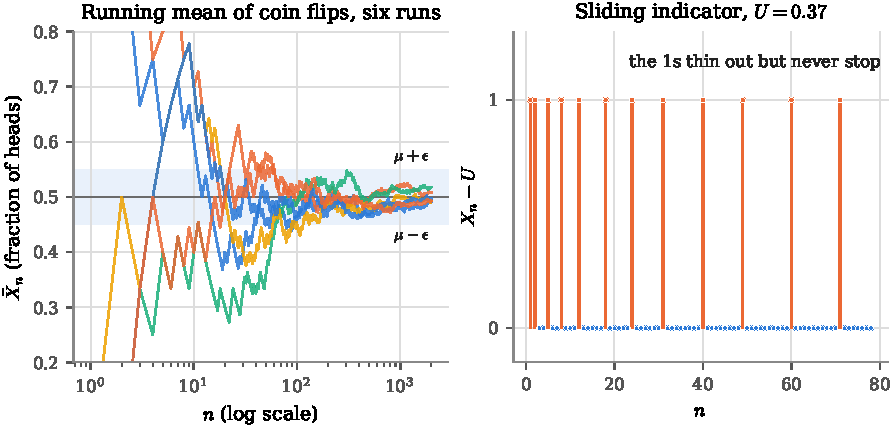
\includegraphics[width=\textwidth]{fig_slln_paths}
\caption{Left: six realizations of the running proportion of heads in a fair coin, on a logarithmic $n$ axis. Each path wanders early, enters the band $\mu \pm 0.05$ and, as the Strong Law says, stays there; with probability one every path eventually does this. Right: one outcome of the sliding-indicator sequence of \cref{ex:sliding}, which converges in probability but not almost surely. For this outcome ($U = 0.37$) the value $1$ keeps recurring, at ever longer intervals, forever.}
\label{fig:sllnpaths}
\end{figure}

\subsection{Convergence almost surely versus convergence in probability}

While the Weak Law of Large Numbers illustrates convergence in probability and the Strong Law of Large Numbers shows convergence almost surely, what's the difference between the two?
The following provides some intuition on the distinction between these two modes of convergence.

Suppose you have some device that improves over time.
So every time you use the device the probability of it failing is less than before.

Convergence in probability says that the chance of failure goes to zero as the number of usages goes to infinity.
So after using the device a large number of times, you can be very confident of it working correctly; it still might fail, but that's very unlikely.

On the other hand, convergence almost surely is a bit stronger.
It says that the total number of failures is \textit{finite}.
That is, if you count the number of failures as the number of usages goes to infinity, you will get a finite number.
The impact of this is as follows: As you use the device more and more, you will, after some finite number of usages, exhaust all failures.
From then on the device will work perfectly.
You don't actually know when you have exhausted all failures, so from a purely practical point of view, there isn't much difference between the two modes of convergence.

It's a good thing that the Strong Law of Large Numbers exists, as opposed to just the Weak Law.
For example, a scientific experiment is justified in taking averages: after obtaining enough data, you can get arbitrarily close to the true average, and there will be only finitely many failures (however improbable) in the averaging process, after which the average stays close.

Here is what `failures (however improbable) in the averaging process' means.
Choose some $\delta > 0$ arbitrarily small.
You obtain $n$ estimates $\Xton$ of some other quantity that has some `true' value, say $\mu$.
You compute the average:
\[
S_n = \frac{1}{n} \sum_{i = 1}^n X_i.
\]

As you obtain more data ($n$ increases) you can compute $S_n$ for $n=1,2,\ldots$.
The Weak Law says (under some assumptions about the $X_n$) that the probability $\Pr( \abs{S_n - \mu } > \delta ) \to 0$, as $n$ goes to $\infty$.
The Strong Law says that the number of times that $\abs{S_n - \mu }$ is larger than $\delta$ is finite (with probability 1).
That is, if we define the indicator function $\ind(\abs{S_n - \mu } > \delta )$ that returns one when $\abs{S_n - \mu } > \delta$ and zero otherwise, then
$\ds \sum_{n=1}^{\infty} \ind(\abs{S_n - \mu } > \delta )$ is finite.
This gives you considerable confidence in the value of $S_n$ because it guarantees, with probability 1, the existence of some finite $n_0$ such that $\abs{S_n - \mu } \leq \delta$ for all $n > n_0$.
That is, the average never fails for $n > n_0$.
Note that the Weak Law gives no such guarantee: it says failures become rare, not that they stop.

The following example, from Casella and Berger, is the standard illustration of a sequence for which failures become rare but never stop.

\begin{example}[The sliding indicator]
\label{ex:sliding}
Let $U \sim \text{Unif}([0,1])$ and define
\begin{align*}
X_1 &= U + \ind(U \in [0, 1]), \\
X_2 &= U + \ind(U \in [0, \tfrac12]), \qquad X_3 = U + \ind(U \in [\tfrac12, 1]), \\
X_4 &= U + \ind(U \in [0, \tfrac13]), \qquad X_5 = U + \ind(U \in [\tfrac13, \tfrac23]), \qquad X_6 = U + \ind(U \in [\tfrac23, 1]), \\
&\ \ \vdots
\end{align*}
so the indicator's interval slides across $[0,1]$ in blocks, and the intervals in the $m$-th block have length $1/m$.
Each $X_n$ equals either $U$ or $U + 1$.
\textit{Convergence in probability holds:} for any $0 < \epsilon < 1$, $\Pr(\abs{X_n - U} \geq \epsilon) = \Pr(U \in [a_n, b_n]) = b_n - a_n$, the length of the $n$-th interval, which goes to zero.
So $X_n \convp U$.
\textit{Almost sure convergence fails:} fix any outcome $U = u$.
In every block, exactly one interval (or two, at a shared endpoint) contains $u$, so $X_n(u) - u$ equals $1$ at least once in every block, forever.
The sequence of numbers $X_n(u)$ therefore takes the value $u + 1$ infinitely often and cannot converge to $u$.
This happens for every outcome, so $\Pr(X_n \to U) = 0$, the opposite of what almost sure convergence requires.
The right panel of \cref{fig:sllnpaths} shows one outcome.
\end{example}

In the device analogy, the sliding indicator is a device whose failures get rarer and rarer but never run out.

\section{Convergence in mean}
\label{sec:conv-mean}

There's a fourth mode, which this book needs only in passing but which you've already used: the shrinking-variance criterion of \cref{prop:shrinking-variance} is a statement about it.

\begin{definition}[Convergence in $r$-th mean]
\label{def:convr}
For $r \geq 1$, a sequence $(X_n)_{n \geq 1}$ \textbf{converges in $r$-th mean} (or in $L^r$) to $X$, written $X_n \convr{r} X$, if
\[
\lim_{n \to \infty} \E \left[ \abs{X_n - X}^r \right] = 0.
\]
The case $r = 2$ is called convergence in mean square (or quadratic mean).
\end{definition}

\begin{inwords}
\textbf{In words.} The average size of the error, measured by its $r$-th power, goes to zero. For $r = 2$ this is `the quadratic risk goes to zero'.
\par\smallskip
\textbf{For the kiss data.} $\E[(\bar{R}_n - p)^2] = p(1-p)/n \to 0$, so $\bar{R}_n \to p$ in mean square; by Markov's inequality \toolkit{sec:math-inequalities} that implies convergence in probability, which is the shrinking-variance criterion of \cref{ch:lln} again.
\end{inwords}

Convergence in mean square to a constant $\mu$ is exactly the condition $\E[(X_n - \mu)^2] \to 0$, and since $\E[(X_n - \mu)^2] = \var(X_n) + (\E[X_n] - \mu)^2$ (variance plus squared bias, the identity behind the quadratic risk of \cref{ch:estimators}), it holds if and only if $\E[X_n] \to \mu$ and $\var(X_n) \to 0$.
Convergence in $r$-th mean implies convergence in probability, by Markov's inequality applied to $\abs{X_n - X}^r$:
\[
\Pr(\abs{X_n - X} \geq \epsilon) = \Pr(\abs{X_n - X}^r \geq \epsilon^r) \leq \frac{\E \abs{X_n - X}^r}{\epsilon^r} \to 0.
\]
Neither convergence in mean nor almost sure convergence implies the other.

\section{The hierarchy of convergence types}
\label{sec:conv-hierarchy}

A sequence of r.v.s might converge for one type of convergence, but not for another.
Some convergence types are `stronger' than others by which it's meant that if Type A convergence is stronger than Type B convergence, then Type A convergence implies Type B convergence.
In \cref{fig:hierarchy}, the stronger types of convergence are given at the top and as you move to the bottom the type of convergence becomes weaker.
By way of example, if a sequence of r.v.s converges in probability, then it converges in distribution as well.

\begin{figure}[htbp]
\centering
\begin{tikzpicture}[
  node distance=1.0cm and 1.6cm,
  mode/.style={draw, rounded corners=2pt, minimum width=3.6cm, minimum height=0.9cm, align=center, font=\small, fill=gray!5},
  imp/.style={-{Latex[length=2.5mm]}, thick},
  lbl/.style={font=\scriptsize, fill=white, inner sep=1pt}
]
  \node[mode] (as) {almost surely\\ $X_n \convas X$};
  \node[mode, right=of as] (lr) {in $r$-th mean\\ $X_n \convr{r} X$};
  \node[mode, below=of $(as)!0.5!(lr)$] (p) {in probability\\ $X_n \convp X$};
  \node[mode, below=of p] (d) {in distribution\\ $X_n \convd X$};
  \draw[imp] (as) -- (p);
  \draw[imp] (lr) -- (p);
  \draw[imp] (p) -- (d);
  \draw[imp, dashed, boxorange!80!black] (d.east) to[bend right=50] node[lbl, right] {only if $X$ is a constant} (p.east);
  \node[font=\scriptsize, left=0.2cm of p, align=right, text=gray] {strong};
  \node[font=\scriptsize, left=0.2cm of d, align=right, text=gray] {weak};
\end{tikzpicture}
\caption{The hierarchy. Solid arrows are implications that always hold; no solid arrow reverses. The dashed arrow is the one partial converse that matters: convergence in distribution to a \textit{constant} is the same as convergence in probability to it. Almost sure convergence and convergence in mean don't imply each other.}
\label{fig:hierarchy}
\end{figure}

Why does this hierarchy exist? Let's focus on the 3 main modes of convergence.
Consider the following points:
\begin{itemize}
\item \textbf{Almost sure convergence:} If a sequence of r.v.s converges almost surely to an r.v., it means that the probability of the sequence eventually staying close to the limiting r.v.\ is 1.
This is the strongest form of convergence because it tells us that the individual values of the r.v.s in the sequence will eventually be close to the limiting r.v.\ with probability 1.
Since the sequence eventually stays within $\epsilon$ of the limit, the probability of being more than $\epsilon$ away at time $n$ must go to zero, which is convergence in probability.

\item \textbf{Convergence in probability:} If a sequence of r.v.s converges in probability to an r.v., it means that for any given $\epsilon > 0$, the probability of the difference between the random variables in the sequence and the limiting r.v.\ being greater than $\epsilon$ goes to 0 as the sequence progresses.
This is weaker than almost sure convergence because it only tells us about the probability of the r.v.s being close to the limiting r.v.\ at each $n$ separately, not that they will eventually be close with probability 1.
The sliding indicator of \cref{ex:sliding} is the example of the gap.

\item \textbf{Convergence in distribution:} If a sequence of r.v.s converges in distribution to an r.v., it means that the cumulative distribution functions (CDFs) of the r.v.s in the sequence converge pointwise to the CDF of the limiting r.v.
This is the weakest form of convergence because it only tells us about the behavior of the distribution of the r.v.s, not about the individual values or their probabilities of being close to the limiting r.v.
If $X_n$ is close to $X$ with high probability then their CDFs must be close, which is why convergence in probability implies convergence in distribution; the $X_n = -Z$ example in the pitfall box of \cref{sec:conv-dist} shows the converse fails.
\end{itemize}


The dashed arrow in \cref{fig:hierarchy} is \cref{prop:convd-constant}: convergence in distribution to a constant is convergence in probability to it.


\section{Summary}
\label{sec:modes-summary}

\begin{center}
\small
\begin{tabular}{@{}>{\raggedright\arraybackslash}p{1.45in}>{\raggedright\arraybackslash}p{2.2in}>{\raggedright\arraybackslash}p{2.3in}@{}}
\toprule
Mode & Definition & Where it's used in this book \\
\midrule
almost surely, $X_n \convas X$ & $\Pr(X_n \to X) = 1$ & Strong Law of Large Numbers \\[4pt]
in probability, $X_n \convp X$ & $\Pr(\abs{X_n - X} \geq \epsilon) \to 0$ for every $\epsilon > 0$ & Weak LLN; consistency of estimators; the constant in Slutsky's theorem \\[4pt]
in distribution, $X_n \convd X$ & $F_{X_n}(x) \to F_X(x)$ at every continuity point of $F_X$ & CLT; confidence intervals; test statistics \\[4pt]
in $r$-th mean, $X_n \convr{r} X$ & $\E\abs{X_n - X}^r \to 0$ & shrinking-variance criterion ($r = 2$); quadratic risk \\
\bottomrule
\end{tabular}
\end{center}

\section{Exercise}

\begin{exercise}
Is the following statement correct? `If $(T_n)_{n \geq 1}$ converges in probability, then it also converges almost surely.'
\end{exercise}
\begin{solution}
No. The sliding indicator of \cref{ex:sliding} converges in probability to $U$ and almost surely to nothing.
\end{solution}
